\documentclass [a4paper, 12pt] {article}
\usepackage{tikz}
\usepackage [margin = 2cm] {geometry}
\usepackage{xcolor}
\definecolor{customcolor1}{HTML}{00aeef}
\definecolor{customcolor2}{HTML}{f58220}

\title{Data Structure}
\author{Pranto}
\date{\today}

\begin{document}
\maketitle
\section{Graph 6}
Lets make the Tree of ED task 6.
\begin{center}
    \vspace{10pt}
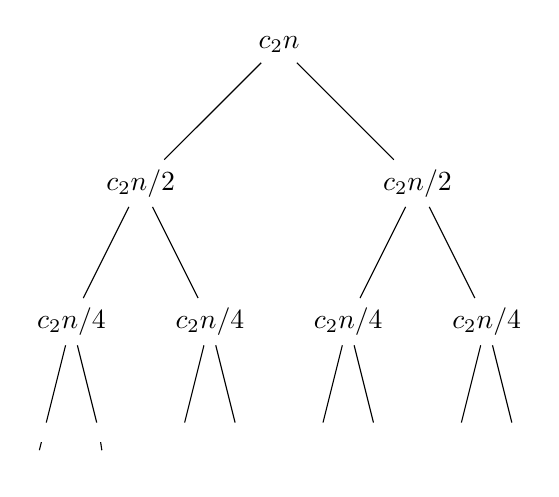
\begin{tikzpicture}
    % Nodes
    \node (a) at (0pt, 0pt) {$c_{2}n$};

    \node (b) at (-50pt, -50pt) {$c_{2}n/2$};
    \node (c) at (50pt, -50pt) {$c_{2}n/2$};

    \node (d) at (-75pt, -100pt) {$c_{2}n/4$};
    \node (e) at (-25pt, -100pt) {$c_{2}n/4$};
    \node (f) at (25pt, -100pt) {$c_{2}n/4$};
    \node (g) at (75pt, -100pt) {$c_{2}n/4$};
%       -75         -25        25          75
%   -85     -65 -35     -15 15      35  65      85
% 
    \node (h) at (-85pt, -140pt) {};
    \node (h1) at (-87.5pt, -150pt) {};
    \node (i) at (-65pt, -140pt) {};
    \node (i1) at (-63.5pt, -150pt) {};
    \node (j) at (-35pt, -140pt) {};
    \node (j1) at (-37.5pt, -150pt) {};
    \node (k) at (-15pt, -140pt) {};
    \node (k1) at (-13.5pt, -150pt) {};
    \node (l) at (15pt, -140pt) {};
    \node (l1) at (13.5pt, -150pt) {};
    \node (m) at (35pt, -140pt) {};
    \node (m1) at (37.5pt, -150pt) {};
    \node (n) at (65pt, -140pt) {};
    \node (n1) at (63.5pt, -150pt) {};
    \node (o) at (85pt, -140pt) {};
    \node (o1) at (87.5pt, -150pt) {};

    \draw[dashed] (h) -- (h1);
    \draw[dashed] (i) -- (i1);


    % Lines
    \draw (a) -- (b) -- (d) -- (h);
    \draw (a) -- (c) -- (g) -- (o);
    \draw (b) -- (e) -- (k);
    \draw (c) -- (f) -- (l);
    \draw (d) -- (i);
    \draw (e) -- (j);
    \draw (f) -- (m);
    \draw (g) -- (n);


\end{tikzpicture}
\end{center}
\end{document}

